\documentclass[tikz]{standalone}
\usepackage{tikz}
\usepackage{pgfplots,graphicx}
\pgfplotsset{compat=newest,compat/show suggested version=false}
\usetikzlibrary{pgfplots.groupplots,matrix}
\usetikzlibrary{positioning,fit,calc,shapes,patterns,automata}
\usepackage{tabularx,xfrac,color,makecell}
\usepackage{array}
\usetikzlibrary{plotmarks}
\usepackage{aurical}
\usepackage[T1]{fontenc}

\usepackage{fontspec}
\setmainfont{Aozora Mincho Regular}

\newcommand{\lmr}{\fontfamily{lmr}\selectfont} % Latin Modern Roman

\tikzset
	{
		tag/.style=
			{
				font=\footnotesize,
				anchor=north west,
				outer sep=0,
				rectangle
			}	
	}
\tikzset
	{
		pron/.style=
			{
				font=\scriptsize,
				anchor=south west,
				outer sep=0,
				draw,
				rectangle,
				ultra thin
			}	
	}
\newcommand{\vier}[4]
	{
		\begin{tabular}{@{}r@{}c@{  }l@{}}
			\textsc{\textbf{\color{red}{#1}}} & $\mathbf{\wr}$ & \textbf{\color{blue}{#2}} \\
			\textsc{#3} & $\wr$ & #4
		\end{tabular}
	}
\begin{document}
\begin{tikzpicture}
\matrix (m) 
	[
		matrix of nodes,
		nodes=
			{
				draw,
				rectangle,
				ultra thick,
				outer sep=0,
				anchor=center,
				minimum height=5cm,minimum width=4cm
			}
	]
	{
		{
\includegraphics[width=4cm]{painting.pdf}} &
		{
\includegraphics[width=4cm]{possible.pdf}} &
		{
\includegraphics[width=4cm]{god.pdf}} &
		{
\includegraphics[width=4cm]{perish.pdf}} &
		{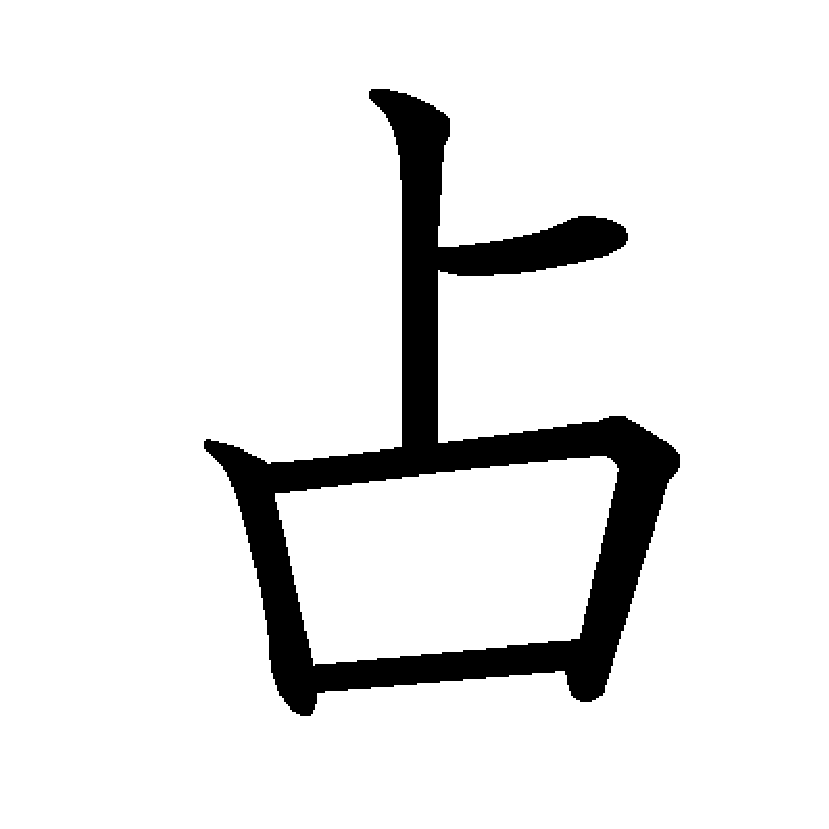
\includegraphics[width=4cm]{occupy.pdf}} \\
		{
\includegraphics[width=4cm]{society.pdf}} &
		{
\includegraphics[width=4cm]{fixed.pdf}} &
		{
\includegraphics[width=4cm]{paper.pdf}} &
		{
\includegraphics[width=4cm]{appearance.pdf}} &
		{
\includegraphics[width=4cm]{army.pdf}} \\
		{
\includegraphics[width=4cm]{elder_sister.pdf}} &
		{
\includegraphics[width=4cm]{sheep.pdf}} &
		{
\includegraphics[width=4cm]{intervene.pdf}} &
		{
\includegraphics[width=4cm]{platform.pdf}} &
		{
\includegraphics[width=4cm]{hasten.pdf}} \\
		{
\includegraphics[width=4cm]{state.pdf}} &
		{
\includegraphics[width=4cm]{spicy.pdf}} &
		{
\includegraphics[width=4cm]{clothes.pdf}} &
		{
\includegraphics[width=4cm]{lucky.pdf}} &
		{
\includegraphics[width=4cm]{utilize.pdf}} \\
		{
\includegraphics[width=4cm]{next.pdf}} &
		{
\includegraphics[width=4cm]{low.pdf}} &
		{
\includegraphics[width=4cm]{filial_piety.pdf}} &
		{
\includegraphics[width=4cm]{tea.pdf}} &
		{
\includegraphics[width=4cm]{profit.pdf}} \\
		{
\includegraphics[width=4cm]{not_yet.pdf}} &
		{
\includegraphics[width=4cm]{end.pdf}} &
		{
\includegraphics[width=4cm]{dipper.pdf}} &
		{
\includegraphics[width=4cm]{play.pdf}} &
		{
\includegraphics[width=4cm]{bean.pdf}} \\
	};
\node [tag] at (m-1-1.north west) {\Fontlukas Painting};
\node [tag] at (m-1-2.north west) {\Fontlukas Possible};
\node [tag] at (m-1-3.north west) {\Fontlukas God};
\node [tag] at (m-1-4.north west) {\Fontlukas Perish};
\node [tag] at (m-1-5.north west) {\Fontlukas Occupy};
\node [tag] at (m-2-1.north west) {\Fontlukas Society};
\node [tag] at (m-2-2.north west) {\Fontlukas Fixed};
\node [tag] at (m-2-3.north west) {\Fontlukas Paper};
\node [tag] at (m-2-4.north west) {\Fontlukas Appearance};
\node [tag] at (m-2-5.north west) {\Fontlukas Army};
\node [tag] at (m-3-1.north west) {\Fontlukas Elder Sister};
\node [tag] at (m-3-2.north west) {\Fontlukas Sheep};
\node [tag] at (m-3-3.north west) {\Fontlukas Intervene};
\node [tag] at (m-3-4.north west) {\Fontlukas Platform};
\node [tag] at (m-3-5.north west) {\Fontlukas Hasten};
\node [tag] at (m-4-1.north west) {\Fontlukas State};
\node [tag] at (m-4-2.north west) {\Fontlukas Spicy};
\node [tag] at (m-4-3.north west) {\Fontlukas Clothes};
\node [tag] at (m-4-4.north west) {\Fontlukas Lucky};
\node [tag] at (m-4-5.north west) {\Fontlukas Utilize};
\node [tag] at (m-5-1.north west) {\Fontlukas Next};
\node [tag] at (m-5-2.north west) {\Fontlukas Low};
\node [tag] at (m-5-3.north west) {\Fontlukas Filial Piety};
\node [tag] at (m-5-4.north west) {\Fontlukas Tea};
\node [tag] at (m-5-5.north west) {\Fontlukas Profit};
\node [tag] at (m-6-1.north west) {\Fontlukas Not yet};
\node [tag] at (m-6-2.north west) {\Fontlukas End};
\node [tag] at (m-6-3.north west) {\Fontlukas Dipper};
\node [tag] at (m-6-4.north west) {\Fontlukas Play};
\node [tag] at (m-6-5.north west) {\Fontlukas Bean};

\node [pron] at (m-1-1.south west) {\vier{ガ; カク}{--}{--}{--}};
\node [pron] at (m-1-2.south west) {\vier{カ}{--}{--}{--}};
\node [pron] at (m-1-3.south west) {\vier{シン; ジン}{かみ}{--}{かん; こう}};
\node [pron] at (m-1-4.south west) {\vier{ボウ}{な}{モウ}{ほろ}};
\node [pron] at (m-1-5.south west) {\vier{セン}{うらな}{--}{し}};
\node [pron] at (m-2-1.south west) {\vier{セ; セイ}{--}{--}{よ}};
\node [pron] at (m-2-2.south west) {\vier{テイ}{さだ}{ジョウ}{--}};
\node [pron] at (m-2-3.south west) {\vier{シ}{かみ}{--}{--}};
\node [pron] at (m-2-4.south west) {\vier{サイ}{--}{--}{--}};
\node [pron] at (m-2-5.south west) {\vier{グン}{--}{--}{--}};
\node [pron] at (m-3-1.south west) {\vier{シ}{あね}{--}{--}};
\node [pron] at (m-3-2.south west) {\vier{--}{ひつじ}{ヨウ}{--}};
\node [pron] at (m-3-3.south west) {\vier{カイ}{--}{--}{--}};
\node [pron] at (m-3-4.south west) {\vier{ダイ; タイ}{--}{--}{--}};
\node [pron] at (m-3-5.south west) {\vier{キュウ}{いそ}{--}{--}};
\node [pron] at (m-4-1.south west) {\vier{シュウ}{--}{--}{す}};
\node [pron] at (m-4-2.south west) {\vier{--}{から}{シン}{--}};
\node [pron] at (m-4-3.south west) {\vier{フク}{--}{--}{--}};
\node [pron] at (m-4-4.south west) {\vier{キチ; キツ}{--}{--}{--}};
\node [pron] at (m-4-5.south west) {\vier{ヨウ}{--}{--}{もち}};
\node [pron] at (m-5-1.south west) {\vier{ジ}{つ; つぎ}{シ}{--}};
\node [pron] at (m-5-2.south west) {\vier{テイ}{ひく}{--}{--}};
\node [pron] at (m-5-3.south west) {\vier{コ}{--}{--}{--}};
\node [pron] at (m-5-4.south west) {\vier{チャ}{--}{サ}{--}};
\node [pron] at (m-5-5.south west) {\vier{リ}{き}{--}{--}};
\node [pron] at (m-6-1.south west) {\vier{ミ}{--}{--}{--}};
\node [pron] at (m-6-2.south west) {\vier{マツ}{--}{バツ}{すえ}};
\node [pron] at (m-6-3.south west) {\vier{ト}{--}{--}{--}};
\node [pron] at (m-6-4.south west) {\vier{ユウ}{あそ}{ユ}{--}};
\node [pron] at (m-6-5.south west) {\vier{--}{まめ}{ズ; トウ}{--}};

\node (webs)
	[
		anchor=south east,
		color=lightgray,
		outer sep=0
	]
		at (m.north east)
	{
		http:{/}{/}kanji.nihongo.cz/home
	};
\node (chap)
	[
		anchor=south west,
		color=black,
		outer sep=0,
		font=\huge
	]
		at (m.north west)
	{
		\textbf{\lmr Chapter 13}
	};
\end{tikzpicture}
\end{document}